% Este documento LaTeX fue diseñado por profesores  del Instituto de Matemáticas 
% de la Universidad de Antioquia (https://www.matematicasudea.co/). Usted puede modificarlo
% y personalizarlo a su gusto bajo los términos de la licencia de documentación libre GNU.
% http://es.wikipedia.org/w/index.php?title=Licencia_de_documentaci%C3%B3n_libre_de_GNU&oldid=15717448

%\documentclass[envcountsect,serif,9pt,t]{beamer}

\documentclass[envcountsect,serif,9pt,t]{beamer}

%\usepackage{scrextend}
%\changefontsizes{8pt}

\usepackage{etex}

% \setbeamertemplate{navigation symbols}{}

% \setbeamertemplate{title page}[default][colsep=-4bp,rounded=false,shadow=\beamer@themerounded@shadow]

% \setbeamertemplate{blocks}[rounded][shadow=false]

% \setbeamertemplate{title page}[default][colsep=-4bp,rounded=true]


% \setbeamertemplate{frametitle}[default][colsep=-4bp,rounded=false,shadow=false]

\usetheme{Frankfurt}

\usepackage{tcolorbox}

\usepackage{lipsum}

% \hypersetup{pdfpagemode=FullScreen}

% \usecolortheme[rgb={0,0.39,0}]{structure}

%\documentclass[serif,9pt]{beamer}
%\usepackage[T1]{fontenc} % Needed for Type1 Concrete
%\usepackage[charter]{mathdesign}

%\usepackage[pdftex]{graphicx}

% https://www.overleaf.com/learn/latex/Spanish
\usepackage[utf8]{inputenc}
\usepackage[spanish, es-tabla]{babel}

\usepackage{amsmath,amssymb}
%\usepackage[dvips]{graphicx}
\usepackage{multicol}
\usepackage{textcomp}
\usepackage[makeroom]{cancel}
\usepackage{multicol}
\usepackage{colortbl}
\usepackage{pstricks,pst-plot}

\usepackage{eso-pic}

%\usepackage{subfig}
\usepackage{xcolor}
%\usepackage{float}

\usepackage{graphicx}

\usepackage{tikz,tkz-euclide,tikz-3dplot}
% \usetikzlibrary{shadows,decorations.pathmorphing,shapes,arrows,patterns,matrix,positioning,plotmarks,shapes.geometric,shapes.arrows,arrows.meta}
\tikzset{>=latex}
%\usetkzobj{all}

\usepackage{gensymb}

\usepackage{cancel}

% Para las tablas nice
% \usepackage{tikz}
% \usepackage{pgfplots}
% \usetikzlibrary{shadows}

% Para gráficas
\usepackage{graphicx}
\usepackage{caption}
\usepackage{subcaption}

% Para justificar texto
\usepackage{ragged2e}
% \justifying

% https://ctan.math.illinois.edu/macros/latex/contrib/longfbox/longfbox.html
\usepackage{longfbox}

\decimalpoint

\definecolor{azul}{RGB}{0,92,162}

\setbeamercolor{structure}{fg=azul}

%%%%%%%%%%%%%%%%%%%%%%%%%%%%% Definiciones %%%%%%%%%%%%%%%%%%%%%%%%%%%%%%%%%

% https://tex.stackexchange.com/questions/53781/how-can-i-include-the-logo-in-some-slides-and-remove-in-others-using-beamer/53783
\newcommand{\nologo}{\setbeamertemplate{logo}{}} % command to set the logo to nothing

% https://tex.stackexchange.com/questions/123924/indexed-letters-inside-circles
\newcommand\encircle[1]{%
	\tikz[baseline=(X.base)] 
	\node (X) [draw, shape=circle, inner sep=0] {\strut #1};}

% http://tex.stackexchange.com/questions/161301/latex-beamer-enumerate-with-manual-numbers
\newcommand{\labelname}[1]{
	\def\insertenumlabel{#1}%
	\usebeamertemplate{enumerate item}%
}

\newenvironment<>{defi}[1]{%
	\begin{actionenv}#2%
		\def\insertblocktitle{#1}%
		\par%
		\mode<presentation>{}
		\usebeamertemplate{block begin}}
	{\par\usebeamertemplate{block end}\end{actionenv}
}

\newenvironment<>{prop}[1]{%
	\begin{actionenv}#2%
		\def\insertblocktitle{#1}%
		\par%
		\mode<presentation>{%
			\setbeamercolor{block title}{fg=white,bg=green!45!black}
			\setbeamercolor{block body}{fg=black,bg=green!4} 
			%        \setbeamercolor{itemize item}{fg=orange!20!black}crist
			%\setbeamertemplate{itemize item}[triangle]
			\setbeamercolor{item projected}{fg=white,bg=green!60!black}
			%        \setbeamercolor{item projected}{fg=white,bg=orange!100}
		}%
		\usebeamertemplate{block begin}}
	{\par\usebeamertemplate{block end}\end{actionenv}
}

\newenvironment<>{obs}[1]{%
	\begin{actionenv}#2%
		\def\insertblocktitle{#1}%
		\par%
		\mode<presentation>{%
			\setbeamercolor{block title}{fg=white,bg=orange!90!black}
			\setbeamercolor{block body}{fg=black,bg=orange!5}
			%        \setbeamercolor{itemize item}{fg=orange!20!black}
			%\setbeamertemplate{itemize item}[triangle]
			\setbeamercolor{item projected}{fg=white,bg=orange!80!black}
			%        \setbeamercolor{item projected}{fg=white,bg=orange!100}
		}%
		\usebeamertemplate{block begin}}
	{\par\usebeamertemplate{block end}\end{actionenv}
}

\newenvironment<>{ejer}[1]{%
	\begin{actionenv}#2%
		\def\insertblocktitle{#1}%
		\par%
		\mode<presentation>{%
			\setbeamercolor{block title}{fg=white,bg=purpura!40!black}
			\setbeamercolor{block body}{fg=black,bg=columbia!5}
			%        \setbeamercolor{itemize item}{fg=orange!20!black}
			%\setbeamertemplate{itemize item}[triangle]
			\setbeamercolor{item projected}{fg=white,bg=purpura!40!black}
		}%
		\usebeamertemplate{block begin}}
	{\par\usebeamertemplate{block end}\end{actionenv}
}

\newenvironment<>{ej}[1]{%
	\begin{actionenv}#2%
		\def\insertblocktitle{#1}%
		\par%
		\mode<presentation>{%
			\setbeamercolor{block title}{fg=white,bg=orange!90!black}
			\setbeamercolor{block body}{fg=black,bg=orange!5}
			%        \setbeamercolor{itemize item}{fg=orange!20!black}
			%\setbeamertemplate{itemize item}[triangle]
			\setbeamercolor{item projected}{fg=white,bg=orange!80!black}
			%        \setbeamercolor{item projected}{fg=white,bg=orange!100}
		}%
		\usebeamertemplate{block begin}}
	{\par\usebeamertemplate{block end}\end{actionenv}
}

\newenvironment<>{ejem}[1]{%
	\begin{actionenv}#2%
		\def\insertblocktitle{#1}%
		\par%
		\mode<presentation>{%
			\setbeamercolor{block title}{fg=white,bg=red!40!black}
			\setbeamercolor{block body}{fg=black,bg=columbia!5}
			%        \setbeamercolor{itemize item}{fg=orange!20!black}
			%\setbeamertemplate{itemize item}[triangle]
			\setbeamercolor{item projected}{fg=white,bg=purpura!40!black}
		}%
		\usebeamertemplate{block begin}}
	{\par\usebeamertemplate{block end}\end{actionenv}
}

\newenvironment<>{problock}[1]{%
	\begin{actionenv}#2%
		\def\insertblocktitle{#1}%
		\par%
		\mode<presentation>{%
			\setbeamercolor{block title}{fg=white,bg=orange!50!black}
			\setbeamercolor{block body}{fg=black,bg=olive!30}
			\setbeamercolor{itemize item}{fg=orange!20!black}
			\setbeamertemplate{itemize item}[triangle]
			\setbeamercolor{item projected}{fg=white,bg=orange!20!black}
		}%
		\usebeamertemplate{block begin}}
	{\par\usebeamertemplate{block end}\end{actionenv}
}

% \definecolor{darkred}{rgb}{0.8,0,0}
% 
% \newenvironment<>{ejer}[1]{%
%   \begin{actionenv}#2%
%       \def\insertblocktitle{#1}%
%       \par%
%       \mode<presentation>{%
%        \setbeamercolor{block title}{fg=white,bg=orange!20!black}
% %        \setbeamercolor{block body}{fg=black,bg=olive!50}
%        \setbeamercolor{block body}{fg=black,bg=darkred}
%        \setbeamercolor{itemize item}{fg=orange!20!black}
%        \setbeamertemplate{itemize item}[triangle]
%      }%
%       \usebeamertemplate{block begin}}
%     {\par\usebeamertemplate{block end}\end{actionenv}
% }

% http://tex.stackexchange.com/questions/66655/numbered-definitions-theorems-in-beamer
% \setbeamertemplate{theorems}[numbered]
\setbeamertemplate{theorems}[ams style] 
\setbeamertemplate{caption}[numbered]

% \newtheorem{teo}{Teorema}[section]
% \newtheorem{lema}{Lema}[section]
% \newtheorem{pro}{Proposición}[section]
% \newtheorem{defi}{Definici\'on}[section]
% \newtheorem{ej}{Ejemplo}[section]
% \newtheorem{obs}{Observación}[section]

%\newtheorem{}{Teorema}[section]
%\newtheorem{proposition}[theorem]{Proposición}

\def\R{\mathbb{R}}
\def\r{\mathbb{R}}
\def\rn{\mathbb{R}^n}
\def\u{\mathbf{u}}
\def\u{\mathbf{u}}
\def\v{\mathbf{v}}
\def\w{\mathbf{w}}
\def\x{\mathbf{x}}
\def\y{\mathbf{y}}
\def\p{\mathbb{P}}
\def\f{\mathbb{F}}
\def\N{\mathbb{N}}
\def\n{\mathbb{N}}
\def\q{\mathbb{Q}}
\def\Q{\mathbb{Q}}
\def\c{\mathbb{C}}
\def\C{\mathbb{C}}
\def\z{\mathbb{Z}}
\def\Z{\mathbb{Z}}

\def\sen{\mathop{\mbox{\normalfont sen}}\nolimits}
\def\sign{\mathop{\mbox{\normalfont sign}}\nolimits}
\def\intt{\mathop{\mbox{\normalfont int}}\nolimits}
\def\diag{\mathop{\mbox{\normalfont diag}}\nolimits}
\def\arcsen{\mathop{\mbox{\normalfont arcsen}}\nolimits}
\def\ln{\mathop{\mbox{\normalfont ln}}\nolimits}
\def\tr{\mathop{\mbox{\normalfont tr}}\nolimits}
\def\erf{\mathop{\mbox{\normalfont erf}}\nolimits}
\def\erfc{\mathop{\mbox{\normalfont erfc}}\nolimits}

\def\op{\mathop{\mbox{\normalfont op}}\nolimits}
\def\ady{\mathop{\mbox{\normalfont ady}}\nolimits}
\def\hip{\mathop{\mbox{\normalfont hip}}\nolimits}

% \def\.{\mathop{\mbox{\normalfont .}}\nolimits}
\def\rem{\mathop{\mbox{\normalfont rem}}\nolimits}
\def\divi{\mathop{\mbox{\normalfont div}}\nolimits}
\def\modd{\mathop{\mbox{\normalfont mod}}\nolimits}
\def\oo{\mathop{\mbox{ \normalfont O }}\nolimits}
\def\yy{\mathop{\mbox{ \normalfont Y }}\nolimits}
\def\no{\mathop{\mbox{\normalfont NO }}\nolimits}

%%%%%%%%%%%%%%%%%%%%%%%%%%%%%%%%%%%%%%%%%%%%%%%%%%%%%%%%%%%%%%%%%%%%%%%

\newpsobject{grilla}{psgrid}{subgriddiv=1,griddots=10,gridlabels=6pt}
\newpsobject{grillaA}{psgrid}{subgriddiv=1,griddots=6,gridlabels=0pt,gridcolor=grilla-gray}
\newpsobject{grillaB}{psgrid}{subgriddiv=1,griddots=10,gridlabels=0pt,gridcolor=grilla-gray}

%%%%%%%%%%%%%%%%%%%%%%%%%%%%%%%%%%%%%%%%%%%%%%%%%%%%%%%%%%%%%%%%%%%%%%%%%%%%


\newcommand{\myblue}{\only{\color{blue}}}
\newcommand{\myred}{\only{\color{red}}}
\newcommand{\mypurpura}{\only{\color{purpura}}}
\newcommand{\myorange}{\only{\color{orange}}}
\newcommand{\mymagenta}{\only{\color{magenta}}}
\newcommand{\mycyan}{\only{\color{cyan}}}
\newcommand{\mygreen}{\only{\color{olive}}}
\newcommand{\myyellow}{\only{\color{yellow}}}
\newcommand{\mygray}{\only{\color{gray}}}
\def\colorize<#1>{\temporal<#1>{\color{red!50}}{\color{black}}{\color{black!50}}}

%========================================================

\xdefinecolor{dorado}{cmyk}{0,0.10,0.84,0}
\xdefinecolor{melon}{cmyk}{0,0.29,0.84,0}
\xdefinecolor{naranja}{cmyk}{0,0.42,1,0}
\xdefinecolor{durazno}{cmyk}{0,0.46,0.50,0}
\xdefinecolor{fresa}{cmyk}{0,1,0.50,0}
\xdefinecolor{ladrillo}{cmyk}{0,0.77,0.87,0}
\xdefinecolor{violeta}{cmyk}{0.07,0.90,0,0.34}
\xdefinecolor{columbia}{cmyk}{0.39, 0.13, 0.00, 0.00}
\xdefinecolor{purpura}{cmyk}{0.45,0.86,0,0}
\xdefinecolor{aguamarina}{cmyk}{0.85,0,0.33,0}
\xdefinecolor{esmeralda}{cmyk}{0.91,0,0.88,0.12}
\xdefinecolor{pino}{cmyk}{0.92,0,0.59,0.25}
\xdefinecolor{oliva}{cmyk}{0.64,0,0.95,0.40}
\xdefinecolor{canela}{cmyk}{0.14,0.42,0.56,0}
\xdefinecolor{marron}{cmyk}{0,0.72,1,0.45}
\xdefinecolor{cafe}{cmyk}{0,0.81,1,0.60}
\xdefinecolor{gris-claro}{cmyk}{0,0,0,0.30}
\xdefinecolor{gris-oscuro}{cmyk}{0,0,0,0.50}
\definecolor{darkgreen}{rgb}{0,0.39,0}
\xdefinecolor{darkblue}{rgb}{0,0,0.55}

\definecolor{verde}{HTML}{006400} % ver8de

\definecolor{light-gray}{gray}{0.94}
\definecolor{gris}{gray}{0.92}
\definecolor{grilla-gray}{gray}{0.77}

%========================================================

\def\octave{\mathop{\mbox{\normalfont \hspace{.1em}\texttt{Octave} \hspace{-.3em}\raisebox{.4ex}{}}}\nolimits}
\def\goctave{\mathop{\mbox{\normalfont \hspace{.1em}\texttt{GNU Octave} \hspace{-.3em}\raisebox{.4ex}{}}}\nolimits}

\beamersetuncovermixins{\opaqueness<1>{10}}{\opaqueness<2->{10}}

\begin{document}

\title{Álgebra lineal -- Semana 5 \\[2mm] Cambio de base}
\author{
	% \href{mailto:alejandro.piedrahita@udea.edu.co}{Alejandro Piedrahita H.} \\[6mm]
	\texorpdfstring{Grupo EMAC\newline{\footnotesize \url{grupoemac@udea.edu.co} } }{} \\[6mm]
	Facultad de Ciencias Exactas y Naturales \\[0mm] %\vspace{0.03cm}
	\href{https://www.matematicasudea.co/}{\color{blue}Instituto de Matemáticas} \\[0mm] %\vspace{0.09cm}
	Universidad de Antioquia}

\date{\today}
\logo{\fbox{
\includegraphics[scale=0.12]{imagenes/udea}}} 
%\logo{\fbox{\includegraphics[width=2cm, height=1.4cm]{imagenes/profe}}\phantom{xx} } 

\begin{frame}
 \titlepage
\end{frame}

% Remueve el logo de la página de inicio:
% https://tex.stackexchange.com/questions/56966/prevent-logo-from-title-page-in-beamer-class?rq=1
%\frame[plain]{\titlepage}

%-----------------------------------------------------------------------------------------------------------------


% \begin{frame}
% \frametitle{Contenido}\tableofcontents
% \end{frame} 

%-----------------------------------------------------------------------------------------------------------------

\section{Valores y vectores propios}

\subsection{}

{\nologo 
\begin{frame}\frametitle{Valores y vectores propios de una matriz}

\begin{figure}	
	\begin{subfigure}[b]{0.45\textwidth}
		\centering
		\begin{tikzpicture}[thick,scale=0.7, every node/.style={scale=0.6}]%[scale=.8,font=\scriptsize]
		\draw[help lines,white,dotted] (-3,-2) grid (3,2);
		\draw[thick,-latex] (-3,0) -- (3,0) node[below] {\large $x$};
		\draw[thick,-latex] (0,-2) -- (0,2) node[above] {\large $y$};
		%\fill[color=blue] (0,0) circle[radius=2pt];			
		% Vector v
		\draw [line width=0.4mm,color=blue,->] (0,0) -- (1.5,1);
		\fill[color=blue,draw] (1.5,0.8) node[below] {\Large $\mathbf{v} $};	
		% Vector lambda v
		\draw [line width=0.2mm,color=red,->] (0,0) -- (2.5,1.67);
		\fill[color=red,draw] (2.5,1.5) node[below] {\Large $\lambda\mathbf{v} $};	
		\end{tikzpicture}
		\caption{$\lambda>0$}
	\end{subfigure}
	\hfill
	\begin{subfigure}[b]{0.45\textwidth}
		\centering
		\begin{tikzpicture}[thick,scale=0.7, every node/.style={scale=0.6}]%[scale=.8,font=\scriptsize]
		\draw[help lines,white,dotted] (-3,-2) grid (3,2);
		\draw[thick,-latex] (-3,0) -- (3,0) node[below] {\large $x$};
		\draw[thick,-latex] (0,-2) -- (0,2) node[above] {\large $y$};
		%\fill[color=blue] (0,0) circle[radius=2pt];			
		% Vector v
		\draw [line width=0.3mm,color=blue,->] (0,0) -- (1.5,1);
		\fill[color=blue,draw] (1.5,0.8) node[below] {\Large $\mathbf{v} $};	
		% Vector lambda v
		\draw [line width=0.3mm,color=red,->] (0,0) -- (-2.5,-1.67);
		\fill[color=red,draw] (-1.9,-1.4) node[below] {\Large $\lambda\mathbf{v} $};	
		\end{tikzpicture}
		\caption{$\lambda<0$}
	\end{subfigure}
	%	\caption{Pictures of animals}\label{fig:animals}
\end{figure}

\begin{defi}{\textbf{Definición 1}}\justifying
	\justifying
	Sea $A$ una matriz $n\times n$. Un escalar $\lambda$ (real o complejo) se dice que es un \textbf{\textit{valor propio}}
	de $A$, si existe un vector no nulo $\mathbf{v}$ tal que
	\begin{equation}\label{vp}
		A \mathbf{v} = \lambda \mathbf{v}.
	\end{equation}
	Al vector $\mathbf{v}$ que satisface \eqref{vp} se le denomina \textbf{\textit{vector propio}} de $A$ correspondiente a $\lambda$.
\end{defi}	

\end{frame}
}

%%------------------------------------------------------------------------------------------------------

\subsection{}

{\nologo 
\begin{frame}\frametitle{Valores y vectores propios de una matriz}

\begin{defi}{\textbf{Definición 1}}\justifying
	\justifying
	Sea $A$ una matriz $n\times n$. Un escalar $\lambda$ (real o complejo) se dice que es un \textbf{\textit{valor propio}}
	de $A$, si existe un vector no nulo $\mathbf{v}$ tal que
	\begin{equation}\tag{1}%\label{vp}
	A \mathbf{v} = \lambda \mathbf{v}.
	\end{equation}
	Al vector $\mathbf{v}$ que satisface \eqref{vp} se le denomina \textbf{\textit{vector propio}} de $A$ correspondiente a $\lambda$.
\end{defi}	

\begin{alertblock}{\textbf{Observación 1}}
	\begin{enumerate}[$a$]\justifying
		\item El vector $\mathbf{v}=\mathbf{0}$ no puede ser vector propio de una matriz. \\[2mm]
		\item El escalar $\lambda = 0$ sí puede ser valor propio de una matriz. \\[2mm]
		\item Una matriz puede tener muchos valores propios y repetidos.
		\item A los valores propios de una matriz también se les llama \textbf{\textit{autovalores}}
		o \textbf{\textit{valores característicos}}.
		\item A los vectores propios de una matriz también se les llama \textbf{\textit{autovectores}}
		o \textbf{\textit{vectores característicos}}.
	\end{enumerate}
\end{alertblock}

\end{frame}
}

%%------------------------------------------------------------------------------------------------------

\subsection{}

{\nologo 
\begin{frame}%\frametitle{Valores y vectores propios de una matriz}

\begin{defi}{\textbf{Definición 1}}\justifying
	\justifying
	Sea $A$ una matriz $n\times n$. Un escalar $\lambda$ (real o complejo) se dice que es un \textbf{\textit{valor propio}}
	de $A$, si existe un vector no nulo $\mathbf{v}$ tal que
	\begin{equation}\tag{1}%\label{vp}
	A \mathbf{v} = \lambda \mathbf{v}.
	\end{equation}
	Al vector $\mathbf{v}$ que satisface \eqref{vp} se le denomina \textbf{\textit{vector propio}} de $A$ correspondiente a $\lambda$.
\end{defi}	

\begin{ej}{\textbf{Ejemplo 1}}
	Considere la matriz
	\[
	A =
	\left(
	\begin{array}{rr}
	2 &  0\\[1mm]
	0 & -1
	\end{array}
	\right).
	\]	
	Compruebe que:
	\begin{enumerate}[$a$]
		\item $\mathbf{v}_1=(1,0)$ es un autovector de $A$ correspondiente 
		al autovalor $\lambda_1 = 2$ . \\[2mm]
		\item $\mathbf{v}_2=(0,1)$ es un autovector de $A$ correspondiente 
		al autovalor $\lambda_2 = -1$.
	\end{enumerate}
\end{ej}
\textit{Solución.}

\end{frame}
}

%%------------------------------------------------------------------------------------------------------

\subsection{}

\begin{frame}\frametitle{Valores y vectores propios de una matriz}

%\begin{defi}{\textbf{Definición 1}}\justifying
%	\justifying
%	Sea $A$ una matriz $n\times n$. Un escalar $\lambda$ (real o complejo) se dice que es un \textbf{\textit{valor propio}}
%	de $A$, si existe un vector no nulo $\mathbf{v}$ tal que
%	\begin{equation}\tag{1}%\label{vp}
%	A \mathbf{v} = \lambda \mathbf{v}.
%	\end{equation}
%	Al vector $\mathbf{v}$ que satisface \eqref{vp} se le denomina \textbf{\textit{vector propio}} de $A$ correspondiente a $\lambda$.
%\end{defi}	

\begin{ej}{\textbf{Ejemplo 2}}
	Considere la matriz
	\[
	A =
	\left(
	\begin{array}{rrr}
	1 & -2 & \phantom{-}1 \\[1mm]
	0 &  0 & 0 \\[1mm]
	0 &  1 & 1
	\end{array}
	\right).
	\]	
	Verifique que
	\[
		\mathbf{v}_1=(-3,-1,1) \qquad \text{y} \qquad \mathbf{v}_2=(1,0,0)
	\]
	son vectores propios de $A$ y encuentre sus valores propios correspondientes.
\end{ej}
\textit{Solución.}

\end{frame}

%%------------------------------------------------------------------------------------------------------

\subsection{}

\begin{frame}\frametitle{Valores y vectores propios de una matriz}

%\begin{defi}{\textbf{Definición 1}}\justifying
%	\justifying
%	Sea $A$ una matriz $n\times n$. Un escalar $\lambda$ (real o complejo) se dice que es un \textbf{\textit{valor propio}}
%	de $A$, si existe un vector no nulo $\mathbf{v}$ tal que
%	\begin{equation}\tag{1}%\label{vp}
%	A \mathbf{v} = \lambda \mathbf{v}.
%	\end{equation}
%	Al vector $\mathbf{v}$ que satisface \eqref{vp} se le denomina \textbf{\textit{vector propio}} de $A$ correspondiente a $\lambda$.
%\end{defi}	

\begin{ej}{\textbf{Ejemplo 3}}
	Encuentre los valores propios de la matriz
	\[
	A =
	\left(
	\begin{array}{rr}
	4 & -2 \\[1mm]
	1 &  1
	\end{array}
	\right)
	\]	
	y sus correspondientes vectores propios.
\end{ej}
\textit{Solución.}

\end{frame}

%%------------------------------------------------------------------------------------------------------

\subsection{}

{\nologo 
\begin{frame}\frametitle{Polinomio característico}

\vspace{-2mm}
\begin{defi}{\textbf{Definición 1}}\justifying
	\justifying
	Sea $A$ una matriz $n\times n$. Un escalar $\lambda$ (real o complejo) se dice que es un \textbf{\textit{valor propio}}
	de $A$, si existe un vector no nulo $\mathbf{v}$ tal que
	\begin{equation}\tag{1}%\label{vp}
	A \mathbf{v} = \lambda \mathbf{v}.
	\end{equation}
	Al vector $\mathbf{v}$ que satisface \eqref{vp} se le denomina \textbf{\textit{vector propio}} de $A$ correspondiente a $\lambda$.
\end{defi}	

\vspace{-1mm}
\begin{prop}{\textbf{Propiedad 1}}
	\justifying
	Sea $A$ una matriz $n\times n$. $\lambda$ es un valor propio de $A$ si y sólo si $\det(A-\lambda I)=0$.
\end{prop}	

\vspace{-1mm}
\begin{defi}{\textbf{Definición 2}}\justifying
	\justifying
	Sea $A$ una matriz $n\times n$. El determinante de la matriz $A-\lambda I$ se denota por $p(\lambda)$
	y se denomina el \textbf{\textbf{\textit{polinomio característico}}} de $A$:
	\[
		p(\lambda) = \det(A-\lambda I).
	\]
	La ecuación $p(\lambda) = 0$ se denomina \textbf{\textit{ecuación característica}} de $A$.
\end{defi}	

\end{frame}
}

%%------------------------------------------------------------------------------------------------------

\subsection{}

\begin{frame}%\frametitle{Proceso para encontrar los valores y vectores propios de una matriz}

\begin{ejem}{\textbf{Procedimiento 1}}\justifying
	\justifying
	Sea $A$ una matriz $n\times n$. 
	\begin{enumerate}
		\item Halle el polinomio característico $p(\lambda) = \det(A-\lambda I)$.
		\item Halle las raíces de la ecuación característica $p(\lambda) = \det(A-\lambda I) = 0$.
		\item Resuelva el sistema homogéneo $(A-\lambda_i I) \mathbf{x} = 0$, correspondiente a cada valor propio $\lambda_i$.
	\end{enumerate}
\end{ejem}	

\begin{ej}{\textbf{Ejemplo 4}}
	Encuentre los valores y vectores propios de la matriz
	\[
	A =
	\left(
	\begin{array}{rrr}
	2 & 1 &  0\\[1mm]
	0 & 2 &  0\\[1mm]
	0 & 0 & 2
	\end{array}
	\right)
	\]	
\end{ej}
\textit{Solución.}

\end{frame}

%%------------------------------------------------------------------------------------------------------

\subsection{}

\begin{frame}\frametitle{Propiedades de los valores y vectores propios}
	
	\begin{prop}{\textbf{Propiedad 2}}
		\justifying
		Los valores propios de una matriz triangular son las entradas en su diagonal principal.
	\end{prop}	
		
\end{frame}

%%------------------------------------------------------------------------------------------------------

\subsection{}

\begin{frame}\frametitle{Propiedades de los valores y vectores propios}
	
	\begin{prop}{\textbf{Propiedad 3}}
		\justifying
		Sea $A$ una matriz cuadrada. Entonces $A$ es invertible si y sólo si $0$ \textit{\textbf{no}} es un valor propio de $A$.
	\end{prop}	
	
\end{frame}

%%------------------------------------------------------------------------------------------------------

\subsection{}

\begin{frame}\frametitle{Valores y vectores propios}
	
	\begin{prop}{\textbf{Propiedad 4}}
		\justifying
		Sea $A$ una matriz $n\times n$ con valor propio $\lambda$. Entonces el conjunto 
		\[
		E_{\lambda} = \{ \mathbf{x} \mid A\mathbf{x}=\lambda\mathbf{x} \}
		\]
		es un subespacio.
	\end{prop}		

	
\end{frame}

%%------------------------------------------------------------------------------------------------------

\subsection{}

\begin{frame}\frametitle{Valores y vectores propios}
		
	\begin{defi}{\textbf{Definición 3}}\justifying
		Sea $A$ una matriz $n\times n$ con valor propio $\lambda$. Al subespacio
		\[
		E_{\lambda} = \{ \mathbf{x} \mid A\mathbf{x}=\lambda\mathbf{x} \}
		\]
		se le denomina \textbf{\textit{espacio propio}} o \textbf{\textit{espacio característico}}
		de $\lambda$. A la dimensión de $E_{\lambda}$ se le denomina \textbf{\textit{multiplicidad geométrica}}
		de $\lambda$.
	\end{defi}	

	\begin{alertblock}{\textbf{Observación 2}}
		\[
			E_{\lambda} = \{ \mathbf{x} \mid A\mathbf{x}=\lambda\mathbf{x} \} 
			            = \{ \mathbf{x} \mid (A-\lambda I)\mathbf{x} = \mathbf{0} \}
			            = N_{A-\lambda I}
		\]
	\end{alertblock}
	
\end{frame}

%%------------------------------------------------------------------------------------------------------

\subsection{}

\begin{frame}\frametitle{Valores y vectores propios de una matriz}
	
	\begin{ejem}{\textbf{Procedimiento 1}}\justifying
		\justifying
		Sea $A$ una matriz $n\times n$. 
		\begin{enumerate}
			\item Halle el polinomio característico $p(\lambda) = \det(A-\lambda I)$.
			\item Halle las raíces de la ecuación característica $p(\lambda) = \det(A-\lambda I) = 0$.
			\item Para cada valor propio $\lambda_i$, halle el espacio propio correspondiente $E_{\lambda_i}$.
		\end{enumerate}
	\end{ejem}		
	
\end{frame}

%%------------------------------------------------------------------------------------------------------

\subsection{}

\begin{frame}\frametitle{Valores y vectores propios de una matriz}
		
	\begin{ej}{\textbf{Ejemplo 5}}
		Encuentre los valores y vectores propios de la matriz
		\[
		A =
		\left(
		\begin{array}{rrr}
		1 & 2 & -1\\[1mm]
		1 & 0 &  1\\[1mm]
		4 & -4 & 5
		\end{array}
		\right)
		\]	
	\end{ej}

	\textit{Solución.}
	
\end{frame}

%%------------------------------------------------------------------------------------------------------

\subsection{}

\begin{frame}\frametitle{Valores y vectores propios de una matriz}
	
%	\begin{ejem}{\textbf{Procedimiento 1}}\justifying
%		\justifying
%		Sea $A$ una matriz $n\times n$. 
%		\begin{enumerate}
%			\item Halle el polinomio característico $p(\lambda) = \det(A-\lambda I)$.
%			\item Halle las raíces de la ecuación característica $p(\lambda) = \det(A-\lambda I) = 0$.
%			\item Para cada valor propio $\lambda_i$, halle el espacio propio correspondiente $E_i$.
%		\end{enumerate}
%	\end{ejem}	
	
	\begin{ej}{\textbf{Ejemplo 6}}
		Encuentre los valores y vectores propios de la matriz
		\[
		A =
		\left(
		\begin{array}{rr}
		2 & -1\\[1mm]		
		5 & -2
		\end{array}
		\right)
		\]	
	\end{ej}
	\textit{Solución.}
	
\end{frame}

%%------------------------------------------------------------------------------------------------------

\subsection{}

\begin{frame}\frametitle{Valores y vectores propios de una matriz}	
	
	\begin{prop}{\textbf{Propiedad 5}}
		\justifying
		Sea $A$ una matriz $n\times n$. Si $\lambda_1,\hdots,\lambda_k$ son $k$ valores propios distintos de $A$, entonces los correspondientes
		vectores propios $\mathbf{v}_1,\hdots,\mathbf{v}_k$ son linealmente independientes.
	\end{prop}		
	
\end{frame}

%%------------------------------------------------------------------------------------------------------

\subsection{}

{\nologo 
\begin{frame}\frametitle{Multiplicidad algebraica y geométrica}	
	
	\vspace{-2mm}	
	\begin{alertblock}{\textbf{Observación 3}}
		En el ejemplo 4, la matriz
		\[
		A =
		\left(
		\begin{array}{rrr}
		2 & 1 &  0\\[1mm]
		0 & 2 &  0\\[1mm]
		0 & 0 & 2
		\end{array}
		\right)
		\]	
		tiene polinomio característico $p(\lambda) = -(\lambda-2)^3$ y $\dim E_{\lambda}=2$.
	\end{alertblock}
	
	\begin{defi}{\textbf{Definición 4}}\justifying
		Sea $A$ una matriz cuadrada y sea $\lambda_i$ un valor propio de $A$.
		\begin{enumerate}[$a$]\justifying 
			\item Se dice que $\lambda_i$ es un valor propio de \textbf{multiplicidad algebraica} $k$, si $(\lambda-\lambda_i)^k$ es la mayor potencia que es factor del polinomio característico de $A$.
			\item La \textbf{multiplicidad geométrica} de $\lambda_i$ se define como la dimensión del espacio propio correspondiente a $\lambda_i$, es decir,
			\[
				\text{ multiplicidad geométrica de } \lambda_i = \dim E_{\lambda_i} = \nu(A-\lambda_i I).
			\]
		\end{enumerate}				
	\end{defi}	
	
\end{frame}
}

%%------------------------------------------------------------------------------------------------------

\subsection{}

\begin{frame}\frametitle{Propiedades de los valores y vectores propios}	

\begin{prop}{\textbf{Propiedad 6}}
	\justifying
	Sea $A$ una matriz cuadrada con valor propio $\lambda$. Entonces 
	\[
	\text{multiplicidad geométrica de } \lambda \ \leq \ \text{multiplicidad algebraica de } \lambda.
	\]
\end{prop}	

\begin{prop}{\textbf{Propiedad 7}}
	\justifying
	Sea $A$ una matriz $n\times n$. Entonces 
	\begin{enumerate}[$a$]\justifying
		\item $A$ tiene $n$ vectores propios \textit{linealmente independientes}
		si y solo si la multiplicidad geométrica de todo valor propio de $A$ es igual a la multiplicidad algebraica.
		\item En particular, $A$ tiene $n$ vectores propios \textit{linealmente independientes} si todos sus valores propios son diferentes.
	\end{enumerate}		
\end{prop}	

\end{frame}

%%------------------------------------------------------------------------------------------------------

\subsection{}

\begin{frame}\frametitle{Propiedades de los valores y vectores propios}

\begin{prop}{\textbf{Propiedad 8}}
	\justifying
	Sean $A$ una matriz cuadrada y $\lambda$ un valor propio de $A$, con vector propio correspondiente $\mathbf{x}$.
	Entonces:
	\begin{enumerate}[$a$]\justifying
		\item Para cualquier entero $n>0$, $\lambda^n$ es un valor propio de $A^n$ con vector propio correspondiente
		$\mathbf{x}$.
		\item Si $A$ es invertible, entonces $\frac{1}{\lambda}$ es un valor propio de $A^{-1}$ con vector propio correspondiente 
		$\mathbf{x}$.
		\item Si $A$ es invertible, entonces para cualquier entero $n$, $\lambda^n$ es un valor propio de $A^n$ con vector propio correspondiente
		$\mathbf{x}$.
	\end{enumerate}		
\end{prop}	

\end{frame}

%%------------------------------------------------------------------------------------------------------

\subsection{}

\begin{frame}\frametitle{Propiedades de los valores y vectores propios}
			
	\begin{ej}{\textbf{Ejemplo 7}}\justifying
		La matriz $A$ dada a continuación, tiene valores propios $\lambda_1=-1$ y $\lambda_2=2$, con vectores 
		propios correspondientes $\mathbf{x}_1$ y $\mathbf{x}_2$.
		\[
		A =
		\left(
		\begin{array}{rr}
		0 & 1\\[1mm]		
		2 & 1
		\end{array}
		\right),\quad 
		\mathbf{x}_1 =
		\left(
		\begin{array}{r}
		1\\[1mm]		
		-1
		\end{array}
		\right), \quad 
		\mathbf{x}_2 =
		\left(
		\begin{array}{r}
		1\\[1mm]		
		2
		\end{array}
		\right).
		\]	
		Calcule 
		\[
		\left(
		\begin{array}{rr}
		0 & 1\\[1mm]		
		2 & 1
		\end{array}
		\right)^{10}
		\left(
		\begin{array}{c}
		5\\[1mm]		
		1
		\end{array}
		\right).
		\]
	\end{ej}
	\textit{Solución.}
	
\end{frame}

%%------------------------------------------------------------------------------------------------------

\subsection{}

\begin{frame}\frametitle{Propiedades de los valores y vectores propios}
	
	\begin{prop}{\textbf{Propiedad 9}}
		\justifying
		Suponga que $A$ es una matriz cuadrada que tiene vectores propios $\mathbf{v}_1 , \mathbf{v}_2 ,\hdots,\mathbf{v}_m$, 
		con correspondientes valores propios $\lambda_1,\lambda_2,\hdots,\lambda_m$. Si $\mathbf{x}$ es un vector en 
		$\r^n$ tal que
		\[
			\mathbf{x} = c_1\mathbf{v}_1 + c_2\mathbf{v}_2 + \cdots + c_m\mathbf{v}_m,
		\]
		entonces para cualquier entero $k$, 
		\[
			A^k\mathbf{x} = c_1{\lambda_1}^k\mathbf{v}_1 + c_2{\lambda_2}^k\mathbf{v}_2 + \cdots + c_m{\lambda_m}^k\mathbf{v}_m.
		\]
	\end{prop}	
	
\end{frame}


\section{Modelos poblacionales}

\subsection{}

\begin{frame} 
	
	\begin{ejer}{\textbf{Modelo de crecimiento poblacional}} \justifying
		El crecimiento poblacional de una especie de venados se estudia en base a las hembras que son clasificadas en dos etapas de vida:
		
		\vspace{-2mm}
		\begin{multicols}{2}
			\begin{itemize}
				\item Juvenil: $<1$ año
				\item Adulta: $\ge 1$ año
			\end{itemize}
		\end{multicols}
	
		\vspace{-2mm}
		Las hembras adultas procrean en promedio 1.6 hembras cada año, y cada año sobreviven 30\% de las juveniles y 80\% de las adultas. Al inicio hay 20 juveniles y 100 adultas.
		\begin{enumerate}[$a$]
			\item Determine la población de hembras en cualquier año $k$.
%			\item Cuál es la población 10 años después.
%			\item Muestre que la población crece con el tiempo.
%			\item Se debe controlar el crecimiento de la especie cazando un porcentaje de adultos. Cuánto debe ser el porcentaje de caza para que la población se mantenga estable. 
		\end{enumerate}
	\end{ejer}
	
	\textit{Solución.}
	
	\vspace{2mm}
	
	$j_k$: número de hembras juveniles en el año $k$ (desde el inicio del estudio).
	$a_k$: número de hembras adultas en el año $k$ (desde el inicio del estudio).
	
	\begin{itemize}
		\item Al inicio:
		\[
			j_0={\color{ForestGreen}20} \qquad  \text{y} \qquad  a_0={\color{ForestGreen}100}
		\] 
		
		\item Población 1 año después:
		\[	
		\begin{array}{c@{\hspace{0.7\tabcolsep}}c@{\hspace{0.7\tabcolsep}}r@{\hspace{0.7\tabcolsep}}c@{\hspace{0.7\tabcolsep}}c}
		j_1 & = & 0j_0 & + & 1.6a_0 \\[1mm]
		a_1 & = & 0.3j_0 & + & 0.8a_0 \\
		\end{array}
		\quad \Leftrightarrow \quad 
		\left(
		\begin{array}{@{\hspace{0.2\tabcolsep}}c@{\hspace{0.2\tabcolsep}}}
			j_1 \\[1mm]
			a_1	
		\end{array}
		\right)
		=
		\left(
		\begin{array}{@{\hspace{0.2\tabcolsep}}c@{\hspace{1.2\tabcolsep}}c@{\hspace{0.2\tabcolsep}}}
			0 & 1.6 \\[1mm]
		  0.3 & 0.8
		\end{array}
		\right)
		\left(
		\begin{array}{@{\hspace{0.2\tabcolsep}}c@{\hspace{0.2\tabcolsep}}}
		{\color{ForestGreen}20} \\[1mm]
		{\color{ForestGreen}100}
		\end{array}
		\right)
		\]
	\end{itemize}
	
\end{frame}

%%------------------------------------------------------------------------------------------------------

\subsection{}

\begin{frame}\frametitle{Modelo de crecimiento poblacional}
		
%	$j_k$: número de hembras juveniles en el año $k$ (desde el inicio del estudio).
%	$a_k$: número de hembras adultas en el año $k$ (desde el inicio del estudio).
	
%	\vspace{2mm}
	\begin{itemize}
%		\item Al inicio:
%		\[
%		j_0={\color{ForestGreen}20} \qquad  \text{y} \qquad  a_0={\color{ForestGreen}100}
%		\] 
%		
%		\vspace{2mm}
%		\item En el año 1:
%		\[	
%		\begin{array}{c@{\hspace{0.7\tabcolsep}}c@{\hspace{0.7\tabcolsep}}r@{\hspace{0.7\tabcolsep}}c@{\hspace{0.7\tabcolsep}}c}
%		j_1 & = & 0j_0 & + & 1.6a_0 \\[1mm]
%		a_1 & = & 0.3j_0 & + & 0.8a_0 \\
%		\end{array}
%		\quad \Leftrightarrow \quad 
%		\left(
%		\begin{array}{@{\hspace{0.2\tabcolsep}}c@{\hspace{0.2\tabcolsep}}}
%		j_1 \\[1mm]
%		a_1	
%		\end{array}
%		\right)
%		=
%		\left(
%		\begin{array}{@{\hspace{0.2\tabcolsep}}c@{\hspace{1.2\tabcolsep}}c@{\hspace{0.2\tabcolsep}}}
%		0 & 1.6 \\[1mm]
%		0.3 & 0.8
%		\end{array}
%		\right)
%		\left(
%		\begin{array}{@{\hspace{0.2\tabcolsep}}c@{\hspace{0.2\tabcolsep}}}
%		{\color{ForestGreen}20} \\[1mm]
%		{\color{ForestGreen}100}
%		\end{array}
%		\right)
%		\]
		
		\item  Población 1 año después:
		\[	
		\begin{array}{c@{\hspace{0.7\tabcolsep}}c@{\hspace{0.7\tabcolsep}}r@{\hspace{0.7\tabcolsep}}c@{\hspace{0.7\tabcolsep}}c}
		j_1 & = & 0j_0 & + & 1.6a_0 \\[1mm]
		a_1 & = & 0.3j_0 & + & 0.8a_0 \\
		\end{array}
		\quad \Leftrightarrow \quad 
		\left(
		\begin{array}{@{\hspace{0.2\tabcolsep}}c@{\hspace{0.2\tabcolsep}}}
		j_1 \\[1mm]
		a_1	
		\end{array}
		\right)
		=
		\left(
		\begin{array}{@{\hspace{0.2\tabcolsep}}c@{\hspace{1.2\tabcolsep}}c@{\hspace{0.2\tabcolsep}}}
		0 & 1.6 \\[1mm]
		0.3 & 0.8
		\end{array}
		\right)
		\left(
		\begin{array}{@{\hspace{0.2\tabcolsep}}c@{\hspace{0.2\tabcolsep}}}
		{\color{ForestGreen}20} \\[1mm]
		{\color{ForestGreen}100}
		\end{array}
		\right)
		\]
		
		\vspace{4mm}
		\item Población {\color{red}2} años después: 
		\[	
		\begin{array}{c@{\hspace{0.7\tabcolsep}}c@{\hspace{0.7\tabcolsep}}r@{\hspace{0.7\tabcolsep}}c@{\hspace{0.7\tabcolsep}}c}
		j_2 & = & 0j_1 & + & 1.6a_1 \\[1mm]
		a_2 & = & 0.3j_1 & + & 0.8a_1 \\
		\end{array}
		\quad \Leftrightarrow \quad 
		\left(
		\begin{array}{@{\hspace{0.2\tabcolsep}}c@{\hspace{0.2\tabcolsep}}}
		j_2 \\[1mm]
		a_2	
		\end{array}
		\right)
		=
		\left(
		\begin{array}{@{\hspace{0.2\tabcolsep}}c@{\hspace{1.2\tabcolsep}}c@{\hspace{0.2\tabcolsep}}}
		0 & 1.6 \\[1mm]
		0.3 & 0.8
		\end{array}
		\right)
		\left(
		\begin{array}{@{\hspace{0.2\tabcolsep}}c@{\hspace{0.2\tabcolsep}}}
			j_1 \\[1mm]
			a_1
		\end{array}
		\right)
		\]
		
		\[
		\phantom{	
		\begin{array}{c@{\hspace{0.7\tabcolsep}}c@{\hspace{0.7\tabcolsep}}r@{\hspace{0.7\tabcolsep}}c@{\hspace{0.7\tabcolsep}}c}
		j_2 & = & 0j_1 & + & 1.6a_1 \\[1mm]
		a_2 & = & 0.3j_1 & + & 0.8a_1 \\
		\end{array}
		}
		\ \ \quad \Leftrightarrow \quad 
		\left(
		\begin{array}{@{\hspace{0.2\tabcolsep}}c@{\hspace{0.2\tabcolsep}}}
		j_2 \\[1mm]
		a_2	
		\end{array}
		\right)
		=
		\left(
		\begin{array}{@{\hspace{0.2\tabcolsep}}c@{\hspace{1.2\tabcolsep}}c@{\hspace{0.2\tabcolsep}}}
		0 & 1.6 \\[1mm]
		0.3 & 0.8
		\end{array}
		\right)^{\color{red}2}
		\left(
		\begin{array}{@{\hspace{0.2\tabcolsep}}c@{\hspace{0.2\tabcolsep}}}
		{\color{ForestGreen}20} \\[1mm]
		{\color{ForestGreen}100}
		\end{array}
		\right)
		\]
		
		\vspace{1mm}
		\item Población ${\color{red}k}$ años después: 
		\[	
			\mathbf{u}_k
			\ = \
			\left(
			\begin{array}{@{\hspace{0.2\tabcolsep}}c@{\hspace{0.2\tabcolsep}}}
			j_k \\[1mm]
			a_k	
			\end{array}
			\right)
			=
			\left(
			\begin{array}{@{\hspace{0.2\tabcolsep}}c@{\hspace{1.2\tabcolsep}}c@{\hspace{0.2\tabcolsep}}}
			0 & 1.6 \\[1mm]
			0.3 & 0.8
			\end{array}
			\right)^{\color{red}k}
			\left(
			\begin{array}{@{\hspace{0.2\tabcolsep}}c@{\hspace{0.2\tabcolsep}}}
			{\color{ForestGreen}20} \\[1mm]
			{\color{ForestGreen}100}
			\end{array}
			\right)
			\ = \
			A^{\color{red}k}\mathbf{u}_0
		\]
		
	\end{itemize}
	
\end{frame}

%%------------------------------------------------------------------------------------------------------

\subsection{}

{\nologo
	\begin{frame}\frametitle{Modelo de crecimiento poblacional}
		
		\begin{prop}{\textbf{Problema de la diagonalización}}%{\textbf{Propiedad 9}}
			\justifying
			Si $A$ tiene vectores propios $\mathbf{v}_1$ y $\mathbf{v}_2$, con correspondientes valores propios $\lambda_1$ 
			y $\lambda_2$, entonces
			\[
			\mathbf{u}_0 = c_1\mathbf{v}_1 + c_2\mathbf{v}_2 
			\qquad \Longrightarrow \qquad 
			A^k\mathbf{u}_0 = c_1{\lambda_1}^k\mathbf{v}_1 + c_2{\lambda_2}^k\mathbf{v}_2.
			\]
			
			\vspace{-1mm}
		\end{prop}	
		
		\vspace{2mm}
		\begin{itemize}
			\item El polinomio característico de la \textit{matriz de transición} $A$:
			
			\[	
			p(\lambda)
			=
			|A-\lambda I|
			=
			\left|	
			\begin{array}{@{\hspace{0.2\tabcolsep}}c@{\hspace{1.2\tabcolsep}}c@{\hspace{0.2\tabcolsep}}}
			-\lambda & 1.6 \\[1mm]
			0.3 & 0.8-\lambda
			\end{array}
			\right| 
			=
			(-\lambda)(0.8-\lambda)-0.48
			=
			\lambda^2 - 0.8\lambda - 0.48
			\]
			
			\vspace{4mm}
			\item Los valores propios de la \textit{matriz de transición} $A$:
			
			\[	
			\lambda^2 - 0.8\lambda - 0.48 = (\lambda-1.2)(\lambda+0.4) = 0
			\qquad \Longrightarrow \qquad 
			\lambda=1.2 \quad \text{y} \quad  \lambda=-0.4
			\]
			
		\end{itemize}
		
	\end{frame}
}

%%------------------------------------------------------------------------------------------------------

\subsection{}

\begin{frame}\frametitle{Modelo de crecimiento poblacional}
		
	\begin{itemize}
		\item Espacio propio $E_{\lambda_1}=E_{1.2}=N_{A-1.2I}$:
		
		\[				
			(A-1.2I \ | \ \mathbf{0})
			=
			\left(
			\begin{array}{@{\hspace{0.2\tabcolsep}}r@{\hspace{\tabcolsep}}r@{\hspace{\tabcolsep}}|r@{\hspace{0.2\tabcolsep}}}
			-1.2 & 1.6 & 0  \\[1mm]
			 0.3 & -0.4 & 0
			\end{array}
			\right) 
			\xrightarrow[]{\phantom{xx} }		
			\left(
			\begin{array}{@{\hspace{0.2\tabcolsep}}r@{\hspace{\tabcolsep}}r@{\hspace{\tabcolsep}}|r@{\hspace{0.2\tabcolsep}}}
			0.3 & -0.4 & 0  \\[1mm]
			  0 &    0 & 0
			\end{array}
			\right) 
			\quad \Rightarrow \quad 
			\mathbf{v}_1 = 
			\left(
			\begin{array}{@{\hspace{0.3\tabcolsep}}c@{\hspace{0.5\tabcolsep}}}
				4   \\[1mm]
				3 
			\end{array}
			\right) 
		\]
		
		\vspace{6mm}
		\item  Espacio propio $E_{\lambda_2}=E_{-0.4}=N_{A+0.4I}$:
		
		\[				
		(A+0.4I \ | \ \mathbf{0})
		=
		\left(
		\begin{array}{@{\hspace{0.2\tabcolsep}}r@{\hspace{1.2\tabcolsep}}r@{\hspace{\tabcolsep}}|r@{\hspace{0.2\tabcolsep}}}
		0.4 & 1.6 & 0  \\[1mm]
		0.3 & 1.2 & 0
		\end{array}
		\right) 
		\xrightarrow[]{\phantom{xx} }		
		\left(
		\begin{array}{@{\hspace{0.2\tabcolsep}}r@{\hspace{1.2\tabcolsep}}r@{\hspace{\tabcolsep}}|r@{\hspace{0.2\tabcolsep}}}
		1 & 4 & 0  \\[1mm]
		0 &    0 & 0
		\end{array}
		\right) 
		\quad \Rightarrow \quad 
		\mathbf{v}_2 = 
		\left(
		\begin{array}{@{\hspace{0.3\tabcolsep}}r@{\hspace{0.5\tabcolsep}}}
		-4   \\[1mm]
		 1 
		\end{array}
		\right) 
		\]
		
		\vspace{4mm}
		\item Condiciones iniciales del problema:
		
		\[	
			c_1\mathbf{v}_1 + c_2\mathbf{v}_2 = \mathbf{u}_0
			\quad \Rightarrow \quad 
			\left(
			\begin{array}{@{\hspace{0.2\tabcolsep}}r@{\hspace{1.4\tabcolsep}}r@{\hspace{\tabcolsep}}|c@{\hspace{0.2\tabcolsep}}}
				4 & -4 & {\color{ForestGreen}20}  \\[2mm]
				3 &  1 & {\color{ForestGreen}100}
			\end{array}
			\right) 
			\xrightarrow[]{\phantom{xx} }		
			\left(
			\begin{array}{@{\hspace{0.2\tabcolsep}}r@{\hspace{1.4\tabcolsep}}r@{\hspace{\tabcolsep}}|c@{\hspace{0.2\tabcolsep}}}
			1 & 0 & \frac{105}{4}  \\[2mm]
			0 & 1 & \frac{85}{4}
			\end{array}
			\right)  
		\]
		
	\end{itemize}
	
\end{frame}


%%------------------------------------------------------------------------------------------------------

\subsection{}

\begin{frame}\frametitle{Modelo de crecimiento poblacional}
	
	%	$j_k$: número de hembras juveniles en el año $k$ (desde el inicio del estudio).
	%	$a_k$: número de hembras adultas en el año $k$ (desde el inicio del estudio).
	
	%	\vspace{2mm}
	\begin{itemize}
		
		\vspace{2mm}		
		\item Valores propios:
		
		\[	
			\lambda_1 = 1.2 \qquad \text{y} \qquad \lambda_2 = -0.4
		\]
		
		\vspace{6mm}
		\item Vectores propios:
		
		\vspace{1mm}
		\[	
		\mathbf{v}_1
		\ = \	
		\left(
		\begin{array}{@{\hspace{0.3\tabcolsep}}c@{\hspace{0.5\tabcolsep}}}
		4   \\[1mm]
		3 
		\end{array}
		\right) 
		\qquad \text{y} \qquad
		\mathbf{v}_2
		\ = \	
		\left(
		\begin{array}{@{\hspace{0.3\tabcolsep}}r@{\hspace{0.5\tabcolsep}}}
		-4   \\[1mm]
		1 
		\end{array}
		\right) 
		\]
		
		\vspace{6mm}
		\item $A^{\color{red}k}\mathbf{u}_0 = c_1{\lambda_1}^{\color{red}k}\mathbf{v}_1 + c_2{\lambda_2}^{\color{red}k}\mathbf{v}_2$:
		
		\vspace{1mm}
		\[	
		\mathbf{u}_{\color{red}k}
		\ = \	
		\left(
		\begin{array}{@{\hspace{0.3\tabcolsep}}c@{\hspace{0.5\tabcolsep}}}
		j_k   \\[1mm]
		a_k 
		\end{array}
		\right) 
		\ = \				
		A^{\color{red}k}\mathbf{u}_0
		\ = \
		\frac{105}{4} (1.2)^{\color{red}k}
		\left(
		\begin{array}{@{\hspace{0.3\tabcolsep}}c@{\hspace{0.5\tabcolsep}}}
		4   \\[1mm]
		3 
		\end{array}
		\right) 
		+
		\frac{85}{4} (-0.4)^{\color{red}k}
		\left(
		\begin{array}{@{\hspace{0.3\tabcolsep}}r@{\hspace{0.5\tabcolsep}}}
		-4   \\[1mm]
		1 
		\end{array}
		\right) 
		\]
		
	\end{itemize}
	
\end{frame}

%%------------------------------------------------------------------------------------------------------

\subsection{}

\begin{frame} 
	
	\begin{ejer}{\textbf{Modelo de crecimiento poblacional}} \justifying
		El crecimiento poblacional de una especie de venados se estudia en base a las hembras que son clasificadas en dos etapas de vida:
		
		\vspace{-2mm}
		\begin{multicols}{2}
			\begin{itemize}
				\item Juvenil: $<1$ año
				\item Adulta: $\ge 1$ año
			\end{itemize}
		\end{multicols}
		
		\vspace{-2mm}
		Las hembras adultas procrean en promedio 1.6 hembras cada año, y cada año sobreviven 30\% de las juveniles y 80\% de las adultas. Al inicio hay 20 juvenilese y 100 adultas.
		\begin{enumerate}[$b$]
			%\item Determine la población de hembras en cualquier año $k$.
			\item ¿Cuál es la población 10 años después?
			%\item Muestre que la población crece con el tiempo.
			%\item Se debe controlar el crecimiento de la especie cazando un porcentaje de adultos. Cuánto debe ser el porcentaje de caza para que la población se mantenga estable. 
		\end{enumerate}
	\end{ejer}
	
	\textit{Solución.}
	
	\vspace{0mm}
	
	\begin{prop}{}
	\[	
	%\mathbf{u}_{\color{red}k}
	%\ = \	
	\left(
	\begin{array}{@{\hspace{0.3\tabcolsep}}c@{\hspace{0.5\tabcolsep}}}
	j_k   \\[1mm]
	a_k 
	\end{array}
	\right) 
	%\ = \				
	%A^{\color{red}k}\mathbf{u}_0
	\ = \
	\frac{105}{4} (1.2)^{\color{red}k}
	\left(
	\begin{array}{@{\hspace{0.3\tabcolsep}}c@{\hspace{0.5\tabcolsep}}}
	4   \\[1mm]
	3 
	\end{array}
	\right) 
	+
	\frac{85}{4} (-0.4)^{\color{red}k}
	\left(
	\begin{array}{@{\hspace{0.3\tabcolsep}}r@{\hspace{0.5\tabcolsep}}}
	-4   \\[1mm]
	1 
	\end{array}
	\right) 
	\]
	\end{prop}

	\[		
	p_{\color{red}k}  
	\ = \
	j_{\color{red}k} + a_{\color{red}k}
	\ = \	
	7\cdot \frac{105}{4}\cdot 1.2^{\color{red}k}	
	-
	3\cdot \frac{85}{4}\cdot (-0.4)^{\color{red}k}	
	\]
	
	\vspace{1mm}
	\[		
	p_{\color{red}10}  
	\ = \
	j_{\color{red}10} + a_{\color{red}10}
	\ = \	
	7\cdot \frac{105}{4}\cdot 1.2^{\color{red}10}	
	-
	3\cdot \frac{85}{4}\cdot 0.4^{\color{red}10}
	\ \approx \
	1138
	\]
\end{frame}

%%------------------------------------------------------------------------------------------------------

\subsection{}

\begin{frame} 
	
	\begin{ejer}{\textbf{Modelo de crecimiento poblacional}} \justifying
		El crecimiento poblacional de una especie de venados se estudia en base a las hembras que son clasificadas en dos etapas de vida:
		
		\vspace{-2mm}
		\begin{multicols}{2}
			\begin{itemize}
				\item Juvenil: $<1$ año
				\item Adulta: $\ge 1$ año
			\end{itemize}
		\end{multicols}
		
		\vspace{-2mm}
		Las hembras adultas procrean en promedio 1.6 hembras cada año, y cada año sobreviven 30\% de las juveniles y 80\% de las adultas. Al inicio hay 20 juvenilese y 100 adultas.
		\begin{enumerate}[$c$]
			%\item Determine la población de hembras en cualquier año $k$.
			%\item ¿Cuál es la población 10 años después?
			\item ¿Qué ocurre con la población a medida que pasan los años?
			%\item Se debe controlar el crecimiento de la especie cazando un porcentaje de adultos. Cuánto debe ser el porcentaje de caza para que la población se mantenga estable. 
		\end{enumerate}
	\end{ejer}
	
	\textit{Solución.}
	
	\vspace{2mm}
			
	\begin{prop}{}
	\[		
	p_{\color{red}k}  
	\ = \
	j_{\color{red}k} + a_{\color{red}k}
	\ = \	
	7\cdot \frac{105}{4}\cdot 1.2^{\color{red}k}	
	-
	3\cdot \frac{85}{4}\cdot (-0.4)^{\color{red}k}	
	\]
	\end{prop}
	
	\vspace{4mm}
	\[		
	p_{\color{red}k}  
	%\ = \
	%j_{\color{red}10} + a_{\color{red}10}
	\ = \	
	7\cdot \frac{105}{4}\cdot 1.2^{\color{red}k}	
	-
	3\cdot \frac{85}{4}(-0.4)^{\color{red}k}
	\ \to \
	\infty 
	\qquad \text{cuando} \qquad
	{\color{red}k} \to \infty 
	\]
\end{frame}

%%------------------------------------------------------------------------------------------------------

\subsection{}

\begin{frame} 
	
	\begin{ejer}{\textbf{Modelo de crecimiento poblacional}} \justifying
		El crecimiento poblacional de una especie de venados se estudia en base a las hembras que son clasificadas en dos etapas de vida:
		
		\vspace{-2mm}
		\begin{multicols}{2}
			\begin{itemize}
				\item Juvenil: $<1$ año
				\item Adulta: $\ge 1$ año
			\end{itemize}
		\end{multicols}
		
		\vspace{-2mm}
		Las hembras adultas procrean en promedio 1.6 hembras cada año, y cada año sobreviven 30\% de las juveniles y 80\% de las adultas. Al inicio hay 20 juvenilese y 100 adultas.
		\begin{enumerate}[$d$]
			%\item Determine la población de hembras en cualquier año $k$.
			%\item ¿Cuál es la población 10 años después?
			%\item ¿Qué ocurre con la población a medida que crece con el tiempo?
			\item Se debe controlar el crecimiento de la especie cazando un porcentaje de adultos. ¿Cuánto debe ser el porcentaje de caza para que la población se mantenga estable?
		\end{enumerate}
	\end{ejer}
	
	\textit{Solución.}	
	
	\vspace{1mm}
	
	{\color{red}$h$}: proporción de caza de venados hembra de edad adulta.
	
	\vspace{1mm}
	\begin{itemize}
		\item Población de hembras adultas $k$ años después:
		\[
			a_k \ = \ 0.3\,j_{k-1} + (0.8-{\color{red}h})\,a_{k-1}
		\] 
		
		\vspace{1mm}
		\item La \textit{matriz de transición} resultante es:
		\[	
		A_{\color{red}h} =
		\left(
		\begin{array}{@{\hspace{0.2\tabcolsep}}c@{\hspace{1.6\tabcolsep}}c@{\hspace{0.2\tabcolsep}}}
		0 & 1.6 \\[1mm]
		0.3 & 0.8-{\color{red}h}
		\end{array}
		\right)		
		\]
	\end{itemize}
	
\end{frame}

%%------------------------------------------------------------------------------------------------------

\subsection{}

{\nologo 
\begin{frame}%\frametitle{Modelo de crecimiento poblacional}
			
	\begin{itemize}
		\item Población de hembras adultas $k$ años después:
		\[
		a_k \ = \ 0.3\,j_{k-1} + (0.8-{\color{red}h})\,a_{k-1}
		\] 
		
		\vspace{2mm}
		\item La \textit{matriz de transición} resultante es:
		\[	
		A_{\color{red}h} =
		\left(
		\begin{array}{@{\hspace{0.2\tabcolsep}}c@{\hspace{1.6\tabcolsep}}c@{\hspace{0.2\tabcolsep}}}
		0 & 1.6 \\[1mm]
		0.3 & 0.8-{\color{red}h}
		\end{array}
		\right)		
		\]				
	\end{itemize}
	
	\vspace{-2mm}
	\begin{prop}{\textbf{Condición de estabilidad para la población}}%{\textbf{Propiedad 9}}
		\justifying
		Suponga que $A_{\color{red}h}$ tiene valores propios $\lambda_1$ y $\lambda_2$.
		
		\begin{enumerate}[$a$]
			\item Si $|\lambda_1|<1$ y $|\lambda_2|<1$, entonces
			\[
			\mathbf{u}_k = 
			c_1{\lambda_1}^k\mathbf{v}_1 + c_2{\lambda_2}^k\mathbf{v}_2  \to \mathbf{0}
			\quad \text{cuando} \quad k\to \infty 			
			\]
			y así la población tiende a extinguirse.
			
			\vspace{2mm}
			\item Si $|\lambda_i|>1$ para algún $i$, entonces $\lambda_i\to \infty$ cuando $k\to \infty$ y 
			en tal caso la población aumenta sin control.
			
			\vspace{2mm}
			\item Para que la población se mantenga estable se necesita que $|\lambda_i|=1$.
		\end{enumerate}		
		
		\vspace{-1mm}
	\end{prop}	
	
\end{frame}
}

%%------------------------------------------------------------------------------------------------------

\subsection{}

\begin{frame}%\frametitle{Modelo de crecimiento poblacional}
	
	\begin{itemize}

		\item El polinomio característico de la \textit{matriz de transición} $A_{\color{red}h}$:
		
		\vspace{-1mm}
		\[	
		p(\lambda)
		=
		|A_{\color{red}h}-\lambda I|
		=
		\left|	
		\begin{array}{@{\hspace{0.2\tabcolsep}}c@{\hspace{1.6\tabcolsep}}c@{\hspace{0.2\tabcolsep}}}
		-\lambda & 1.6 \\[1mm]
		0.3 & 0.8-{\color{red}h}-\lambda
		\end{array}
		\right| 
		=
		\lambda^2 - (0.8-{\color{red}h})\lambda - 0.48	
		\]
		
		\vspace{2mm}
		\item Los valores propios de la \textit{matriz de transición} $A_{{\color{red}h}}$:
		
		\vspace{1mm}
		\[	
		\lambda = \frac{0.8-{\color{red}h} \pm \sqrt{( 0.8-{\color{red}h} )^2 - 4\cdot 1\cdot (-0.48) }}{2}
		\]
		
		\vspace{2mm}
		\item Valor de ${\color{red}h}$ para la estabilidad de la población:
		
		\vspace{1mm}
		\[
		\begin{array}{@{\hspace{0.2\tabcolsep}}r@{\hspace{1.6\tabcolsep}}c@{\hspace{1.6\tabcolsep}}l@{\hspace{0.2\tabcolsep}}}
			\dfrac{0.8-{\color{red}h} + \sqrt{( 0.8-{\color{red}h} )^2 - 4\cdot 1\cdot (-0.48) }}{2} & = & 1 \\[4mm]
			%0.8-{\color{red}h} + \sqrt{( 0.8-{\color{red}h} )^2 - 4\cdot 1\cdot (-0.48) } & = & 2 \\[4mm]		
			                     \sqrt{( 0.8-{\color{red}h} )^2 - 4\cdot 1\cdot (-0.48) } & = & 1.2+{\color{red}h} \\[4mm]
			                     ( 0.8-{\color{red}h} )^2 - 4\cdot 1\cdot (-0.48)  & = & (1.2+{\color{red}h})^2 \\[0mm]	
			                     	                                               & \vdots & \\[0mm]
			                     	                                {\color{red}h} & = & 0.28 \ \ = \ \ 28\%
		\end{array}
		\]
	\end{itemize}
	
\end{frame}

%%------------------------------------------------------------------------------------------------------

\subsection{}

{\nologo
\begin{frame} 
	
	\begin{ejer}{\textbf{La sucesión de Fibonacci}} \justifying
		En 1202, Leonardo Fibonacci, también llamado Leonardo de Pisa planteó el siguiente problema: 
		un par de  conejos comienzan a procrear a la edad de un mes, y a partir de ese momento tienen como
		descendencia una nueva pareja de conejos cada mes. Si comenzamos con un par de
		conejos y ninguno de los conejos nacidos a partir de este par muere, ¿cuántos pares
		de conejos tendremos al principio de cada mes?
	\end{ejer}
	
	\textit{Solución.}
	
	\vspace{1mm}
	
	$x_n$: número de parejas de conejos \textbf{al inicio} del mes $n$.
	
	\vspace{3mm}
	
	\begin{columns}[t]
		\hspace{-10mm}
		\begin{column}{0.5\textwidth}
			\vspace{-2mm}
			\begin{itemize}
				\item[] 
\includegraphics[scale=0.25]{imagenes/off}: pareja que no puede procrear. \\[2mm]
				\item[] 
\includegraphics[scale=0.25]{imagenes/on}: pareja que puede procrear.
			\end{itemize}
		\end{column}
		\hspace{-1cm}
		\begin{column}{0.4\textwidth}	
			\vspace{-10mm}
			\centering
			\begin{table}[H]
				\centering
				\begin{tabular}{| c | m{3cm} | c |}
					\hline
					$n$ & Parejas de conejos & $x_n$ \\
					\hline
					&  \vspace{1mm} 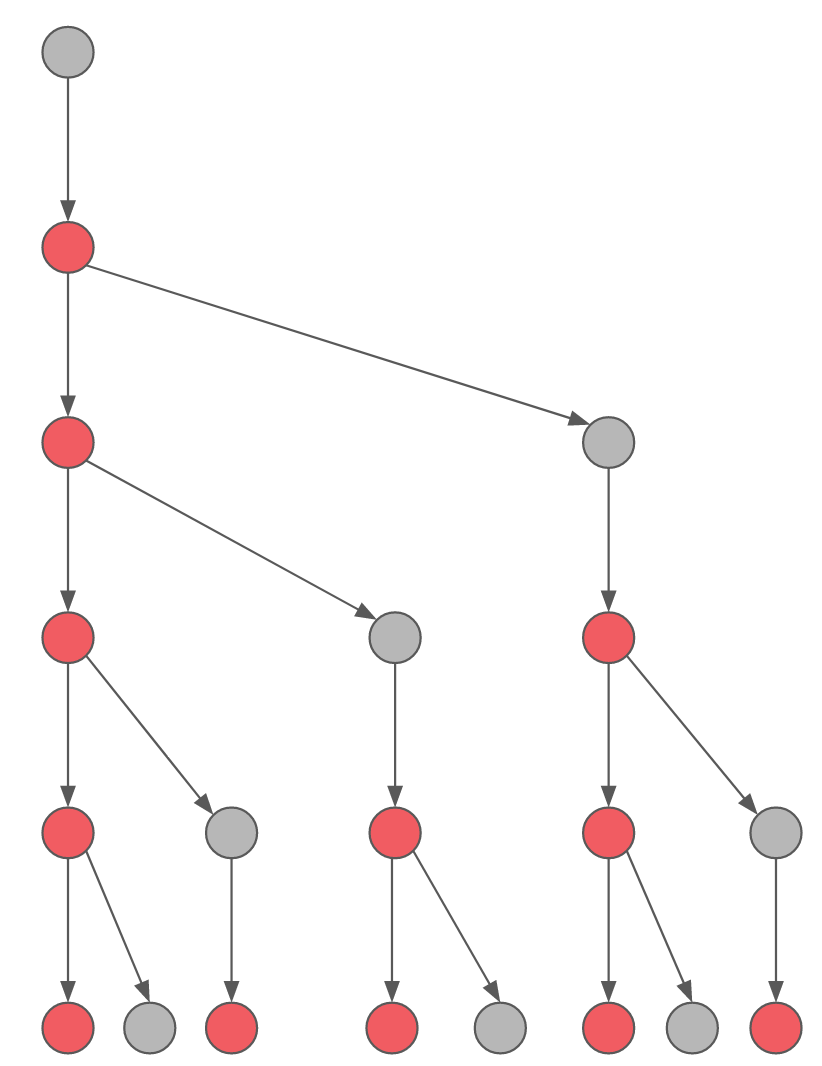
\includegraphics[scale=0.18]{imagenes/fibonacci} &  \\
					\hline
				\end{tabular}
			\end{table}
		\end{column}
		
	\end{columns}
	
\end{frame}
}

%%------------------------------------------------------------------------------------------------------

\subsection{}

{\nologo
	\begin{frame} %\frametitle{Sucesión de Fibonacci}
		
		%$x_n$: número de parejas de conejos \textbf{al inicio} del mes $n$.
		
		\vspace{2mm}
		
		\begin{columns}[t]
			\hspace{-3mm}
			\begin{column}{0.4\textwidth}	
				\vspace{-10mm}
				\centering
				\begin{table}[H]
					\centering
					\begin{tabular}{| c | m{3cm} | c |}
						\hline
						$n$ & Parejas de conejos & $x_n$ \\
						\hline
						&  \vspace{1mm} 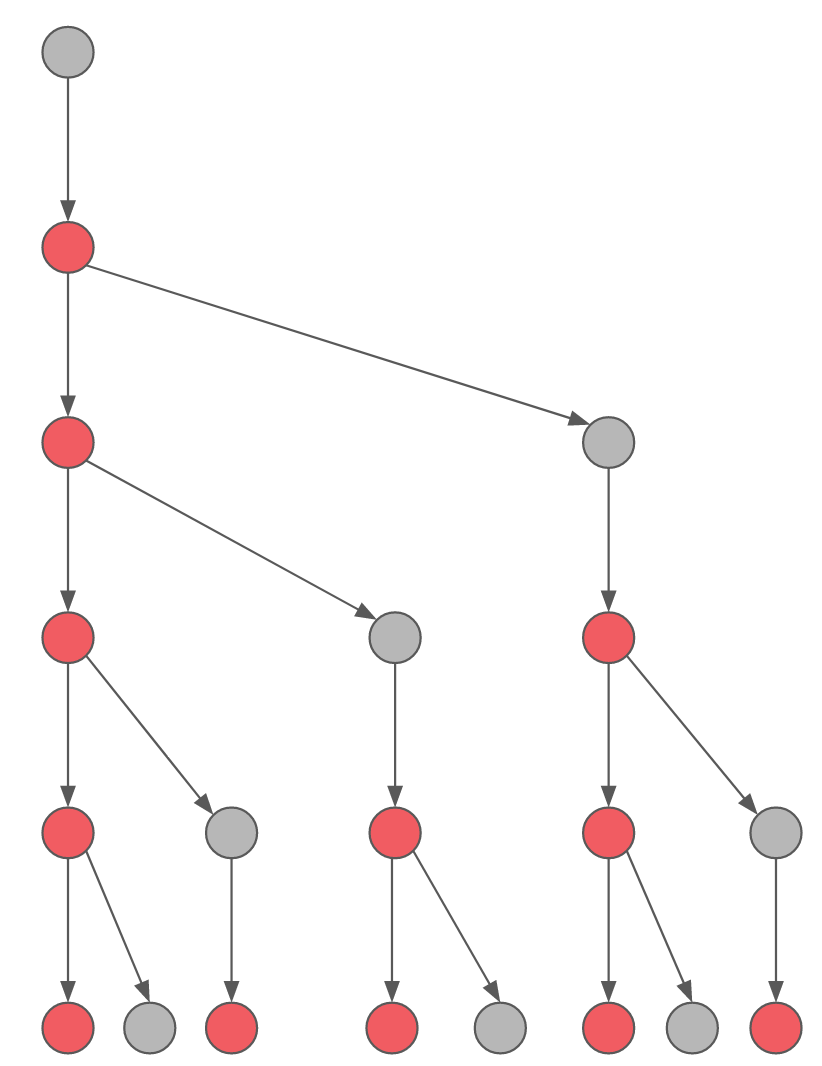
\includegraphics[scale=0.18]{imagenes/fibonacci} &  \\
						\hline
					\end{tabular}
				\end{table}
			\end{column}
			\hspace{-0mm}
			\begin{column}{0.5\textwidth}
				\vspace{-2mm}
				\begin{itemize}
					\item[] 
\includegraphics[scale=0.25]{imagenes/off}: pareja que no puede procrear. \\[2mm]
					\item[] 
\includegraphics[scale=0.25]{imagenes/on}: pareja que puede procrear.
				\end{itemize}
				
				\vspace{0mm}
				\begin{alertblock}{}
					\[
					\begin{array}{c@{\hspace{0.7\tabcolsep}}c@{\hspace{0.7\tabcolsep}}c@{\hspace{0.7\tabcolsep}}c@{\hspace{0.7\tabcolsep}}l}
					x_{n+1}   & = & x_{n}  & + & x_{n-1} \\[2mm]
					x_{n} & = & x_{n},  &   & n=1,2,\hdots  \\[3mm]
					\end{array}
					\]
					
				\end{alertblock}
			\end{column}		
			
		\end{columns}
		
		\vspace{1mm}
		\[
		\left(
		\begin{array}{c}
		x_{n+1}   \\[1mm]
		x_{n} 
		\end{array}
		\right)
		=
		\left(
		\begin{array}{cc}
		1 & 1   \\[1mm]
		1 & 0
		\end{array}
		\right)
		\left(
		\begin{array}{c}
		x_{n}   \\[1mm]
		x_{n-1} 
		\end{array}
		\right)
		\quad \Longrightarrow \quad 
		\mathbf{x}_n = A\, \mathbf{x}_{n-1}
		\]
		%\[
		%\hspace{7mm} \Longrightarrow \quad 
		%\mathbf{x}_n = A\ \mathbf{x}_{n-1}
		%\]
		
		\vspace{-2mm}
		
		\begin{columns}[c]
			\hspace{-10mm}
			\begin{column}{0.5\textwidth}
				\[			
				\begin{array}{c@{\hspace{0.7\tabcolsep}}c@{\hspace{0.7\tabcolsep}}c@{\hspace{0.7\tabcolsep}}c@{\hspace{0.7\tabcolsep}}c@{\hspace{0.7\tabcolsep}}c@{\hspace{0.7\tabcolsep}}c}
				\mathbf{x}_1 & = & A \mathbf{x}_0  &  &  &  & \\[2mm]
				\mathbf{x}_2 & = & A \mathbf{x}_1  & = & A\left( A\mathbf{x}_0\right)  & = & A^2 \mathbf{x}_0\\[2mm]
				\mathbf{x}_3 & = & A \mathbf{x}_2  & = & A\left( A^2\mathbf{x}_0\right)  & = & A^3 \mathbf{x}_0\\[0mm]
				& \vdots &  &  &  &  & \\
				\mathbf{x}_n & = & A^n \mathbf{x}_0  &  &  &  & \\[0mm]             
				\end{array}
				\]	
			\end{column}
			\hspace{-1.2cm}
			\begin{column}{0.1\textwidth}
				\[
				\Longrightarrow
				\]
			\end{column}
			\hspace{-1cm}		
			\begin{column}{0.4\textwidth}	
				\vspace{1mm}
				\[			
				% \mathbf{x}_n = A^n \mathbf{x}_0 
				\left(
				\begin{array}{c}
				x_{n+1}   \\[1mm]
				x_{n} 
				\end{array}
				\right)
				=
				\left(
				\begin{array}{cc}
				1 & 1   \\[1mm]
				1 & 0
				\end{array}
				\right)^n
				\left(
				\begin{array}{c}
				x_{1}   \\[1mm]
				x_{0} 
				\end{array}
				\right)
				\]
			\end{column}
			
		\end{columns}
		
	\end{frame}
}

% ---------------------------------------------------------------------------------------------------

\subsection{}
%
\begin{frame}\frametitle{La sucesión de Fibonacci}
	
	\begin{ej}{\textbf{Ejemplo 1}}\justifying
		Considere la sucesión de Fibonacci
		\[
		1, 1, 2, 3, 5, 8, 13,\hdots {\color{blue}x_n},\hdots
		\]
		
		\vspace{-2mm}
		\begin{enumerate}[$a$]\justifying 
			\item Encuentre una fórmula explícita para hallar el término ${\color{blue}x_n}$ de la sucesión de Fibonacci
			\item ¿A qué valor se aproxima $x_{n+1}/x_n$ cuando $n\to \infty$?
		\end{enumerate}
	\end{ej}
	%\textit{Solución.}
	% https://en.wikipedia.org/wiki/Fibonacci_number#Matrix_form
	% Problema 11 (Poole): https://books.google.com.co/books?id=J4FwdwtfmPAC&lpg=PA446&ots=MU6_Wm8k0I&dq=Con%20su%20respuesta%20al%20problema%2010%2C%20ofrezca%20una%20deducci%C3%B3n%20alternativa%20de%20la%20f%C3%B3rmula%20de%20Binet%20%5Bf%C3%B3rmula%20(5)%20de%20la%20secci%C3%B3n%204.6%5D%3A&hl=es&pg=PA446#v=onepage&q&f=false
	
\end{frame}


 
\section{Referencias}

%\begin{frame}[allowframebreaks,c]\frametitle{Bibliografía}
\begin{frame}\frametitle{Bibliografía}

\begin{thebibliography}{99}

\setbeamertemplate{bibliography item}[book]
\bibitem[]{mejia}
Clara Mejía
\newblock {\em Álgebra lineal elemental y aplicaciones}
\newblock Ude@, 2006.

\vspace{2mm}

\setbeamertemplate{bibliography item}[book]
\bibitem[]{grossman}
Stanley Grossman
\newblock {\em Álgebra lineal}
\newblock McGraw-Hill Interamericana, Edición 8, 2019. 

\vspace{2mm}

\setbeamertemplate{bibliography item}[book]
\bibitem[]{poole}
David Poole
\newblock {\em Álgebra lineal: una introducción moderna}
\newblock Cengage Learning Editores, 2011. 

\vspace{2mm}

\setbeamertemplate{bibliography item}[book]
\bibitem[]{Kolman}
Bernard Kolman
\newblock {\em Álgebra lineal}
\newblock Pearson Educación, 2006.

\vspace{2mm}

\setbeamertemplate{bibliography item}[book]
\bibitem[]{Larson}
Ron Larson
\newblock {\em Fundamentos de Álgebra lineal}
\newblock Cengage Learning Editores, 2010. 

\end{thebibliography}


\end{frame}




\end{document}